\documentclass[10pt, handout]{beamer}
\usepackage[italian]{babel}
\usepackage[utf8]{inputenc}
\usepackage[T1]{fontenc}

\title{Consistency and Replication}
\author{Bartolomeo Lombardi \\ Amerigo Mancino \\ Andrea Segalini}
\date{10 novembre 2015}

\theoremstyle{definition}
\newtheorem{definizione}{Definizione}

\usetheme{Antibes}
%\useoutertheme[right]{sidebar}
\setbeamercovered{dynamic}

\begin{document}

{ % to delimit a block (we only want to remove the header for this frame)
\makeatletter % to change template
    \setbeamertemplate{headline}[default] % not mandatory, but I though it was better to set it blank
    \def\beamer@entrycode{\vspace*{-\headheight}} % here is the part we are interested in :)
\makeatother
\begin{frame}
	\maketitle
\end{frame}
}

\section{COPS}
\begin{frame}
\frametitle{Sistema ALPS}
	\begin{definizione}
	Un \textbf{sistema ALPS} è un sistema caratterizzato da 4 proprietà:
	\begin{itemize}
		\item<1-> Availability
		\item<2-> Low Latency
		\item<3-> Partition-tolerance
		\item<4-> High Scalability
	\end{itemize}
	\end{definizione}
\end{frame}

\begin{frame}
\frametitle{Struttura di COPS}
	\begin{figure}
		\centering
		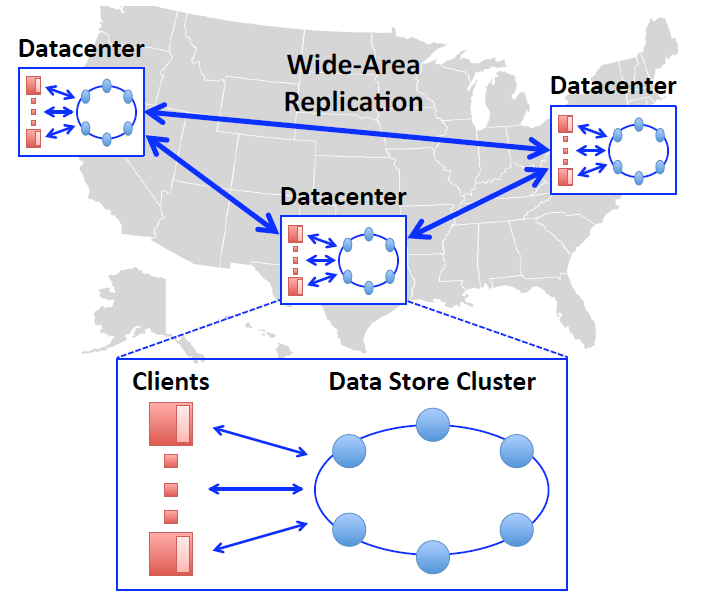
\includegraphics[scale=0.45]{COPS1.png}
	\end{figure}
\end{frame}

\begin{frame}
\frametitle{Potenziale di causalità}
	\begin{definizione}
	Definiamo il \textbf{potenziale di causalità} fra operazioni (e lo denotiamo con $\rightsquigarrow$)
	mediante tre regole:
	\begin{itemize}
		\item<1-> Se $a$ e $b$ sono due operazioni in un singolo thread di esecuzione
				  allora $a \rightsquigarrow b$ se l'operazione $a$ accade prima dell'operazione $b$;
		\item<2-> Se $a$ è un'operazione di \texttt{put} e $b$ è un'operazione di
				  \texttt{get} che ritorna il valore scritto da $a$, allora $a \rightsquigarrow b$;
		\item<3-> Date tre operazioni $a$, $b$, $c$, se $a \rightsquigarrow b$ e $b 
				  \rightsquigarrow c$, allora $a \rightsquigarrow c$.
	\end{itemize}
	\end{definizione}
\end{frame}

\begin{frame}
\frametitle{Un esempio}
	\begin{figure}
		\centering
		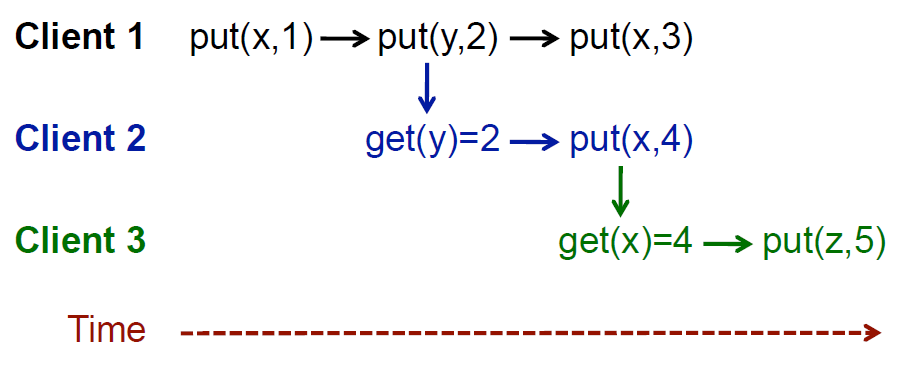
\includegraphics[scale=0.40]{COPS2.png}
	\end{figure}
\end{frame}

\begin{frame}
\frametitle{Casual Consistency +}
\begin{definizione}
Definiamo la \textbf{Causal Consistency +} implementata da COPS come una combinazione di due proprietà:
	\begin{itemize}
		\item<1-> Causal Consistency \\
				  I valori restituiti da un'operazione di \texttt{get} da una replica sono 
				  consistenti con l'ordine definito da $\rightsquigarrow$;
		\item<2-> Convergent conflict handling \\
				  Tutte le operazioni di \texttt{put} in conflitto vengono gestite nello
				  stesso modo da tutte le repliche, usando una funzione di gestione $h$.
	\end{itemize}
\end{definizione}

\begin{definizione}
Si dice che due operazioni $a$ e $b$ sono in conflitto se sono entrambe
due operazione di \texttt{put} sulla stessa chiave.
\end{definizione}
\end{frame}

\begin{frame}
\frametitle{Consistenze a confronto}
	\begin{figure}
		\centering
		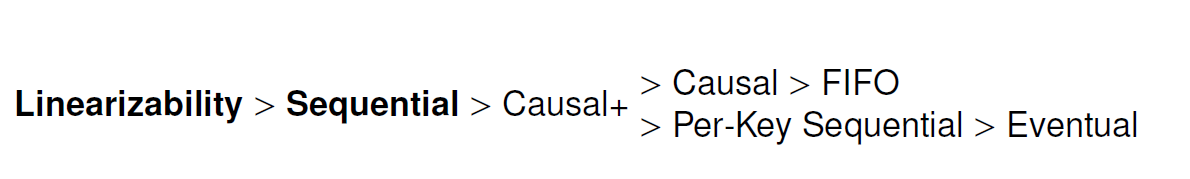
\includegraphics[scale=0.35]{COPS6.png}
	\end{figure}

Se in Amazon Dynamo abbiamo una consistenza che può oscillare fra Strong, Weak, Eventual,
in COPS la definizione risulta più netta: si cerca di implementare il meglio che si può
avere con le caratteristiche ALPS.
\end{frame}

\begin{frame}
\frametitle{Astrazioni di COPS}
\begin{block}{Versione}
Ci riferiamo a differenti valori di una data chiave come alla loro \textbf{versione}
(e la indichiamo con $\text{key}_{version}$).
\end{block}
% Una volta che una data replica in COPS ritorna un certo valore di una data chiave,
% siamo assicurati per Casual Consistency + che i successivi valori richiesti a quella
% replica di quella data chiave saranno quello ottenuto o una sua versione successiva,
% mai precedente
\begin{block}{Dipendenze}
Diciamo che $y_i$ \textbf{dipende da} $x_i$ se e solo se \texttt{put}$(x_i)
\rightsquigarrow$ \texttt{put}$(y_i)$.
\end{block}
\end{frame}

\begin{frame}
\frametitle{Gestione dei conflitti}
\begin{block}{Conflict handling}
COPS può gestire conflitti in diversi modi a seconda dell'implementazione:
	\begin{itemize}
		\item<1-> Last-writer-win-rule \\
				  (detta Thomas Write rule e basata su Timestamp);
				  % La regola dice che se TS(T) < WTS(O), la corrente azione di scrittura è stata resa 
				  % obsoleta dalla più recente operazione di scrittura di O, che segue la scrittura corrente 
				  % basandosi sull'ordinamento del Timestamp.
		\item<2-> Marking dei conflitti e risoluzione con altri mezzi.
	\end{itemize}
\end{block}
Non vengono usati i Vector Clock come invece avviene in Amazon Dynamo perché
si ritiene che in un sistema troppo grande potrebbero andare fuori controllo.
\end{frame}

\begin{frame}
\frametitle{Panoramica di COPS}
\begin{block}{Struttura di COPS}
COPS è formato da due componenti principali:
\begin{itemize}
	\item<1-> Key-value store
	\item<2-> Client library
\end{itemize}
\end{block}
\begin{figure}
	\centering
	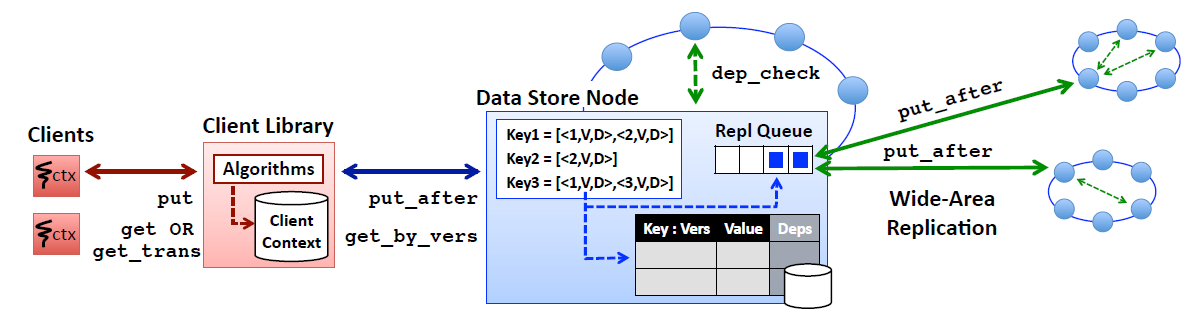
\includegraphics[scale=0.35]{COPS7.png}
\end{figure}
\end{frame}
% Ogni coppia key-value ha associati dei matadati: in COPS questi metadati sono il numero
% di versione, mentre in COPS-GT sono il numero di versione e una lista delle dipendenze
% (ossia una lista di chiavi con la corrispondente versione da cui si dipende)

\begin{frame}
\frametitle{Client library}
L'interfaccia di COPS è composta da quattro operazioni (più una):
\begin{itemize}
	\item<1-> \textit{ctx\char`_id} $\leftarrow$ \texttt{createContext()}
	\item<2-> \textit{bool} $\leftarrow$ \texttt{deleteContext}\textit{(ctx\char`_id)}
	\item<3-> \textit{bool} $\leftarrow$ \texttt{put}\textit{(key, value, ctx\char`_id)}
	\item<4-> \textit{value} $\leftarrow$ \texttt{get}\textit{(key, ctx\char`_id)}
	\item<5-> \textit{values} $\leftarrow$ \texttt{get\char`_trans}\textit{(keys, ctx\char`_id)}
\end{itemize}
\begin{figure}
	\centering
	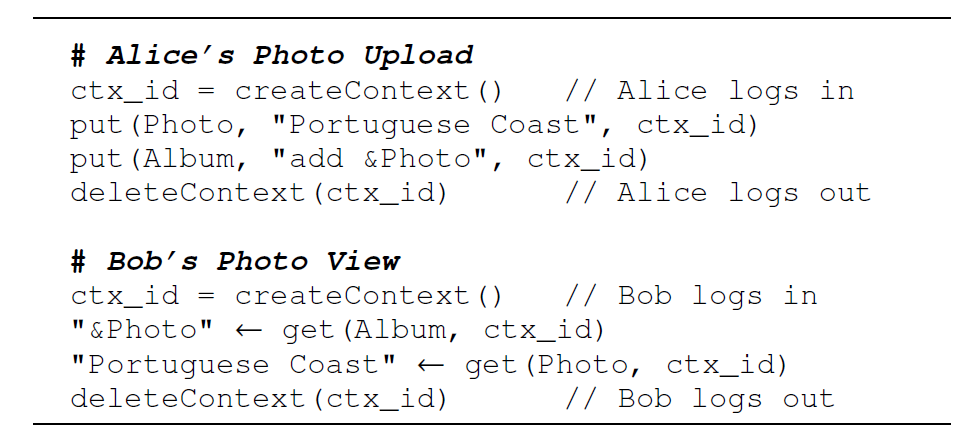
\includegraphics[scale=0.35]{COPS3.png}
\end{figure}
\end{frame}
% Il contesto mi permette di separare e riconoscere i diversi thread di esecuzione
% Il contesto contiene anche le dipendenze fra le variabili

\begin{frame}
\frametitle{Un esempio di dipendenze}
Vediamo un esempio di contesto di un thread all'interno di COPS
(riferito nel nostro caso a $z_4$):
\begin{figure}
	\centering
	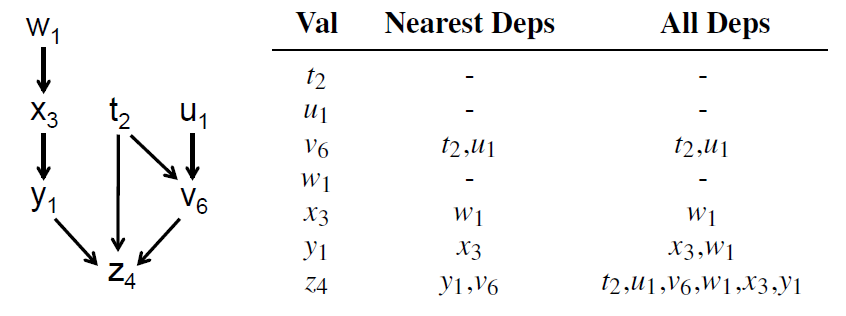
\includegraphics[scale=0.35]{COPS4.png}
\end{figure}
\end{frame}

\begin{frame}
\frametitle{Get Transaction}
\begin{block}{Limiti di COPS}
Leggere un insieme di chiavi dipendenti usando una singola operazione di \texttt{get}
non assicura una consistenza causal+, anche se il data store implementa esso stesso
una politica di causal+ consistency.
\end{block}
\begin{block}{Novità di COPS-GT}
COPS-GT offre un'operazione di \texttt{get\char`_trans} che permette di
ritornare una visione consistente di più chiavi.
\end{block}
\end{frame}

\begin{frame}
\frametitle{Pseudocodice}
Presentiamo un esempio di pseudocodice della \texttt{get\char`_trans}:
\begin{figure}
	\centering
	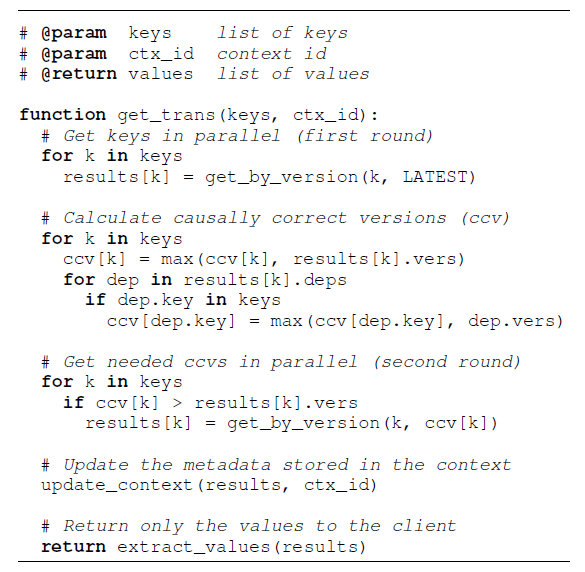
\includegraphics[scale=0.40]{COPS5.png}
\end{figure}
\end{frame}

\end{document}